\documentclass[11pt,a4paper]{article}

\usepackage[margin=0.88in]{geometry}
\usepackage[T1]{fontenc}
\usepackage{lmodern}
\usepackage{amsmath,amssymb,amsfonts}
\usepackage{xcolor}
\usepackage{tikz}
\usepackage{graphicx}
\usepackage{array}
\usepackage{url}
\usepackage{hyperref}

\hypersetup{
  colorlinks=true,
  linkcolor=blue!60!black,
  citecolor=green!45!black,
  urlcolor=blue!60!black,
  pdftitle={VeriCache: Formally Verified, Location-Transparent Distributed KV Caching Across GPU HBM, Host DRAM, NVMe, and GPUDirect RDMA},
  pdfauthor={VeriCache Authors}
}

% Lightweight booktabs-style table rules without requiring extra cached packages
\newcommand{\toprule}{\noalign{\hrule height 0.9pt}\noalign{\vskip 2pt}}
\newcommand{\midrule}{\noalign{\vskip 2pt}\noalign{\hrule height 0.5pt}\noalign{\vskip 2pt}}
\newcommand{\bottomrule}{\noalign{\vskip 2pt}\noalign{\hrule height 0.9pt}}

% Theorem environments without amsthm dependency
\newtheorem{definition}{Definition}[section]
\newtheorem{invariant}[definition]{Invariant}
\newtheorem{lemma}[definition]{Lemma}
\newtheorem{theorem}[definition]{Theorem}

% Consistent typography helpers (robust in captions/TOC; allow clean wrapping at underscores)
\let\origunderscore\_
\DeclareRobustCommand{\code}[1]{{\ttfamily\ifmmode #1\else\def\_{\origunderscore\hspace{0pt}}#1\fi}}
\newcommand{\VC}{\textsc{VeriCache}}
\newcommand{\MC}{\textsc{Mooncake}}
\newcommand{\LM}{\textsc{LMCache}}
\setlength{\emergencystretch}{3.5em}

\definecolor{vcblue}{RGB}{32,96,168}
\definecolor{mcgreen}{RGB}{44,132,76}
\definecolor{lmamber}{RGB}{196,120,24}
\definecolor{alertred}{RGB}{178,34,34}
\definecolor{tcbgray}{RGB}{242,244,248}
\definecolor{layerfill}{RGB}{236,243,252}
\definecolor{corefill}{RGB}{236,248,240}

\title{\textbf{VeriCache: Formally Verified, Location-Transparent Distributed KV Caching Across GPU HBM, Host DRAM, NVMe, and GPUDirect RDMA}}

\author{
  \textbf{VeriCache Technical Report} \\
  \small Revision \code{f476bf7} \quad---\quad November 2026
}

\date{}

\begin{document}
\maketitle

\begin{abstract}
Disaggregated large language model (LLM) inference relies on multi-tier key-value (KV) caches spanning GPU high-bandwidth memory (HBM), pinned host DRAM, local NVMe storage, and cross-node RDMA / GPUDirect RDMA (GDR) pools. Because asynchronous CUDA streams, Linux \code{io\_uring} direct I/O, and one-sided RDMA reads execute outside CPU load/store coherency, cache eviction races silently corrupt shared KV tensors---most acutely when a donor node overwrites a frame while an initiator's NIC still holds an active static remote key (\code{rkey}). Common systems folklore assumes that eliminating such races via formal verification either incurs prohibitive runtime overhead or remains confined to small single-node prototypes.

We present \textbf{\VC{}}, a formally verified, location-transparent distributed KV cache engineered in Verus/Rust. \VC{} decomposes verification across three TCB-audited layers: (1)~\code{vericache-foundation}, a pure concurrency model of fenced asynchronous access histories proving race-freedom and read-last-write equivalence under unilateral revocation; (2)~\code{vericache-transfer}, a slot-granular linear ownership layer (\code{SlotLoc + SlotRef + Seq<u8>}) enforcing a quarantine-on-revoke Type-2B Memory Window (\code{MW}) dynamic lease protocol and mandatory GPUDirect BAR1 visibility flushes; and (3)~\code{vericache-core}, a hardware-free storage kernel (\code{CacheCore}) and composable 4-tier \code{DistributedEngine} using zero-\code{unsafe} Rust borrows and modular \code{core\_transition} frame preservation.

Across the workspace, \textbf{1,210 verification items} (\textbf{69,764~LoC}) pass \emph{both} \code{Z3~4.16.0} and \code{CVC5~1.3.4} (\code{--no-cheating} enforced on \code{vericache-core}), gated by 10 \code{tree-sitter-verus} \code{ast-grep} structural checks that confine \code{unsafe} and \code{external\_body} to an exact \textbf{9-file, 2,151-LoC trusted computing base (3.0\% of system code)}. On dual NVIDIA H20 GPUs and BlueField-3 ConnectX-7 RoCEv2 hardware against production FAST'25 Kimi traces, \VC{} eliminates all 39 silent tearing corruptions exhibited by static-\code{rkey} RDMA under forced eviction, amortizes Type-2B \code{MW} isolation tax to \textbf{+9.9\%} at 4~MB and \textbf{+2.9\%} at 16~MB, and scales to a full \textbf{600~GiB 2-node 4-tier cluster} at \textbf{50.93--72.16~GB/s} (\textbf{1.57$\times$--2.07$\times$} faster than \MC{}~\code{0.3.14} and \textbf{3.83$\times$--4.31$\times$} faster than \LM{}~\code{0.5.7.post1}), with zero leaked scratch files and sub-second-overhead per-tier initialization.
\end{abstract}

\tableofcontents
\clearpage

% ============================================================================
\section{Introduction}
\label{sec:intro}
% ============================================================================

Long-context LLM inference and agentic tool-use workloads transform KV caches from ephemeral per-request scratchpads into shared, latency-critical distributed state~\cite{vllm,mooncake,lmcache}. Because attention keys and values across shared system prompts, RAG prefixes, and multi-turn tool trajectories routinely exceed single-GPU HBM capacity, modern serving engines stripe KV prefixes across a four-tier hierarchy: local GPU HBM, pinned host DRAM, local NVMe solid-state drives, and remote peer HBM/DRAM accessed over one-sided RDMA and GPUDirect RDMA (GDR).

Operating a four-tier cache concurrently exposes a subtle concurrency hazard: \emph{non-coherent asynchronous hardware reclamation races}. When a cache node serves a prefix block to a remote peer over RDMA \code{IBV\_WR\_RDMA\_READ} while simultaneously reclaiming its own local frame under capacity pressure, the CPU cache controller, CUDA copy engine, NVMe DMA engine, and Mellanox RNIC operate on independent timelines. If a donor node unlinks and refills a frame whose static memory region (MR) \code{rkey} remains usable by a slower remote RNIC, the initiator silently reads a prefix-torn hybrid of two distinct prompt contexts---producing undetected corruption in model logits without raising a transport error. Even on a single node, reclaiming a GPU HBM buffer before its consumer CUDA stream retires a downstream kernel, or before \code{cudaHostRegister}-pinned DRAM completes NVMe \code{O\_DIRECT} spill, violates read-last-write integrity.

Existing systems trade away either end-to-end rigor or hardware isolation. High-performance KV engines (\MC{}, \LM{}) rely on static whole-slab MRs, heuristic reference counting, and cooperative timing assumptions; conversely, prior formally verified storage and distributed systems~\cite{ironfleet,verdi,veribetrfs,daisynfs} target disk blocks or RPC state machines rather than asynchronous GPU streams, \code{io\_uring}, and NIC memory-window fencing, and rarely benchmark directly against tuned C++/CUDA/Python serving engines at hundreds-of-gigabytes scale.

\VC{} demonstrates that mechanical, solver-checked hardware safety and state-of-the-art disaggregated throughput need not conflict. Rather than verifying a monolithic server alongside complex eviction heuristics, \VC{} isolates the entire safety-critical data path---slot ownership, asynchronous completion retirement, provenance certificates, and dynamic Type-2B RDMA capability fencing---into three layered Rust/Verus crates while keeping eviction and routing policies cleanly decoupled.

\paragraph{Summary of Contributions.}
\begin{enumerate}
  \item \textbf{Fenced Asynchronous History Semantics (\code{vericache-foundation}):} A domain-parametric ghost model of asynchronous hardware timelines with unilateral read fencing (\code{read\_fenced\_before}). We prove \code{race\_free}, \code{every\_event\_isolated}, and \code{succeeded\_read\_returns\_last\_write} for executions where conflicting reads are either completed before revocation or fenced by the hardware (\code{rejected\_read}).
  \item \textbf{Slot-Granular Ownership \& Type-2B MW RDMA Isolation (\code{vericache-transfer}):} Linear single-key slot tokens (\code{SlotLoc + SlotRef + Seq<u8>}) that avoid SMT quantifier explosion on multi-megabyte KV blocks, paired with a quarantine-on-revoke IBTA Type-2B Memory Window protocol (\code{IBV\_WR\_BIND\_MW}, \code{IBV\_WR\_LOCAL\_INV} + \code{ibv\_dealloc\_mw}, \code{Quarantined} draining, and QP \code{Error -> Reset -> Reconnect}) plus mandatory post-CQE GPUDirect BAR1 visibility flushes (\code{complete\_gdr\_slot}).
  \item \textbf{Hardware-Free Kernel \& 4-Tier Engine (\code{vericache-core}):} A zero-\code{unsafe} cache kernel (\code{CacheCore}), inductive \code{ValueCertificate} provenance, 64-byte \code{FrameSyncMeta} with $O(1)$ \code{SlidingBitmap} ticket retirement, and three-mode \code{core\_transition} composition powering a unified 4-tier \code{DistributedEngine}.
  \item \textbf{Minimal Audited TCB with Dual-SMT Evidence:} \textbf{1,210 proofs} verified under \emph{both} \code{Z3~4.16.0} and \code{CVC5~1.3.4} (\code{--no-cheating} on \code{vericache-core}), governed by 10 \code{tree-sitter-verus} \code{ast-grep} checks enforcing an exact \textbf{9-file, 2,151-LoC (3.0\%) TCB}.
  \item \textbf{Real-Hardware Suites 1--5 Evaluation up to 600~GiB:} On NVIDIA H20 GPUs and BlueField-3 ConnectX-7 hardware, \VC{} eliminates all 39 silent RDMA tearing corruptions observed in \MC{}~\code{0.3.14}, bounds Type-2B MW isolation overhead to \textbf{+2.9\%--9.9\%} at 4--16~MB chunks, and sustains \textbf{50.93--72.16~GB/s} on full production FAST'25 traces at 600~GiB cluster capacity.
\end{enumerate}

% ============================================================================
\section{Threat Model, Design Principles, and Architecture Overview}
\label{sec:arch}
% ============================================================================

\subsection{Failure and Contention Model}

\VC{} targets trusted intra-cluster multi-GPU LLM inference servers connected over lossless/lossy RoCEv2 or InfiniBand fabrics. We do \emph{not} treat remote peer kernels as Byzantine adversaries forging cryptographic packets; rather, our threat model captures the realistic concurrency and timing hazards of high-throughput disaggregated serving:
\begin{itemize}
  \item \textbf{Reordered and Delayed One-Sided RNIC DMA:} Once an initiator RNIC receives a remote descriptor (\code{addr, len, rkey}), CPU scheduling jitter, PCIe backpressure, or queue depth queueing may delay the actual \code{IBV\_WR\_RDMA\_READ} DMA transaction arbitrarily past the moment the donor node decides to evict and overwrite the underlying frame.
  \item \textbf{Concurrent Multi-Engine Hardware Writes:} On a single host, a GPU D2H copy stream, an NVMe \code{io\_uring} SQE write, and an incoming GPUDirect RDMA pull can touch distinct slots concurrently or attempt to reuse the same physical slot prematurely unless ordered by verified \code{Ticket} retirement.
  \item \textbf{Unilateral Revocation \& Cooperative Release Failures:} Under tight HBM/DRAM pressure, a donor cannot block forever waiting for a straggling or stalled peer initiator to return a cooperative \code{ReadRelease}; the donor must fence the remote access unilaterally at the RNIC before reusing its local storage, while the initiator must detect the resulting transport failure (\code{IBV\_WC\_REM\_ACCESS\_ERR}) without propagating corrupted bytes to inference callers.
\end{itemize}

\subsection{Three-Layer Architecture and Decoupled Policy}

Figure~\ref{fig:arch} illustrates \VC{}'s three-layer crate hierarchy and exact trust boundary, while Table~\ref{tab:loc} quantifies code size and verification coverage at revision \code{f476bf7}.

\begin{figure}[t]
\centering
\resizebox{\textwidth}{!}{%
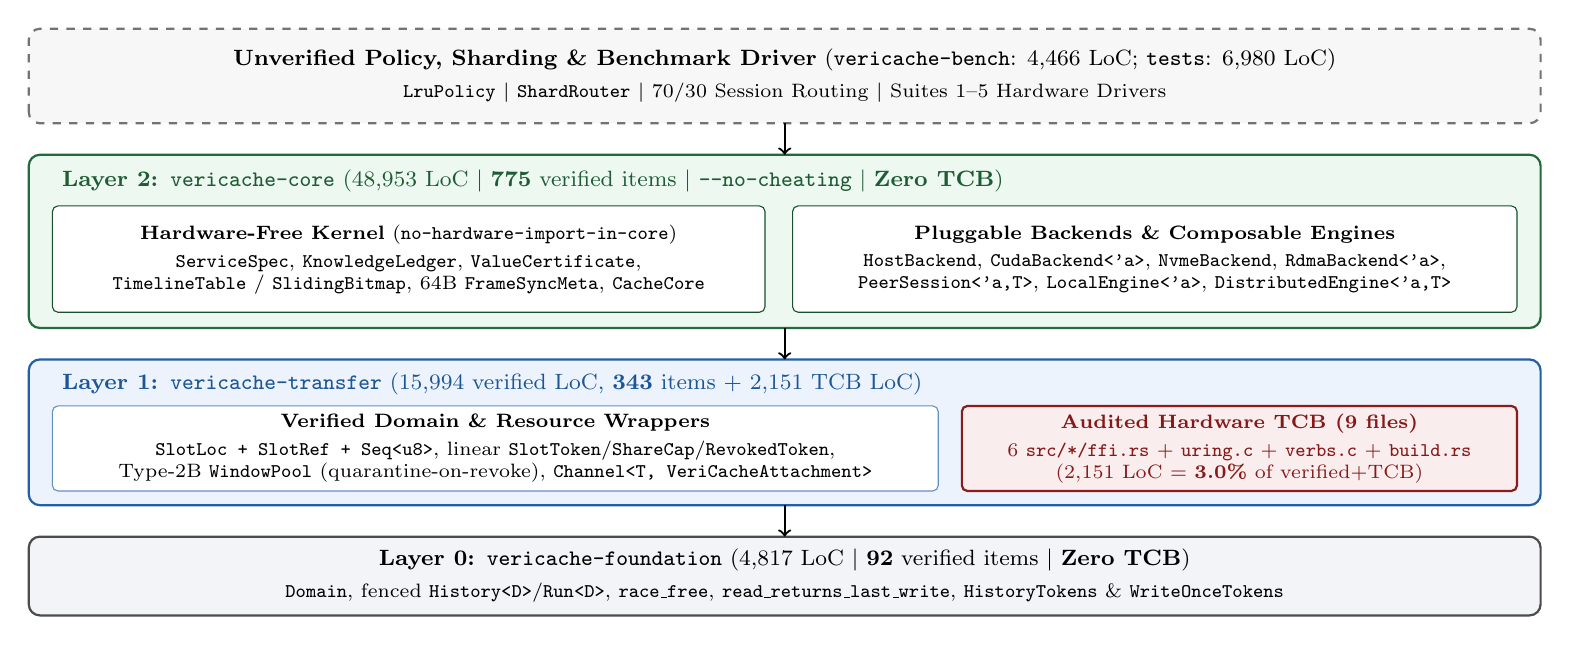
\begin{tikzpicture}[every node/.style={font=\footnotesize}]
  % Top decoupling box: vericache-bench / Policy
  \draw[dashed, thick, draw=black!55, fill=black!3, rounded corners=4pt]
    (0.0, 6.25) rectangle (19.2, 7.45);
  \node[align=center] at (9.6, 6.85) {
    \textbf{Unverified Policy, Sharding \& Benchmark Driver} (\code{vericache-bench}: 4,466 LoC; \code{tests}: 6,980 LoC) \\[2pt]
    \scriptsize \code{LruPolicy} \textbar{} \code{ShardRouter} \textbar{} 70/30 Session Routing \textbar{} Suites 1--5 Hardware Drivers
  };

  % Layer 2: vericache-core
  \draw[thick, draw=mcgreen!80!black, fill=corefill, rounded corners=4pt]
    (0.0, 3.65) rectangle (19.2, 5.85);
  \node[anchor=west, text=mcgreen!70!black] at (0.30, 5.52)
    {\textbf{Layer 2: \code{vericache-core}} (48,953 LoC $\mid$ \textbf{775} verified items $\mid$ \code{--no-cheating} $\mid$ \textbf{Zero TCB})};
  \draw[draw=mcgreen!60!black, fill=white, rounded corners=2pt] (0.30, 3.85) rectangle (9.35, 5.20);
  \node[align=center, font=\scriptsize] at (4.825, 4.52) {
    \textbf{Hardware-Free Kernel} (\code{no-hardware-import-in-core}) \\[2pt]
    \code{ServiceSpec}, \code{KnowledgeLedger}, \code{ValueCertificate}, \\
    \code{TimelineTable} / \code{SlidingBitmap}, 64B \code{FrameSyncMeta}, \code{CacheCore}
  };
  \draw[draw=mcgreen!60!black, fill=white, rounded corners=2pt] (9.70, 3.85) rectangle (18.90, 5.20);
  \node[align=center, font=\scriptsize] at (14.30, 4.52) {
    \textbf{Pluggable Backends \& Composable Engines} \\[2pt]
    \code{HostBackend}, \code{CudaBackend<'a>}, \code{NvmeBackend}, \code{RdmaBackend<'a>}, \\
    \code{PeerSession<'a,T>}, \code{LocalEngine<'a>}, \code{DistributedEngine<'a,T>}
  };

  % Layer 1: vericache-transfer
  \draw[thick, draw=vcblue, fill=layerfill, rounded corners=4pt]
    (0.0, 1.40) rectangle (19.2, 3.25);
  \node[anchor=west, text=vcblue!90!black] at (0.30, 2.94)
    {\textbf{Layer 1: \code{vericache-transfer}} (15,994 verified LoC, \textbf{343} items + 2,151 TCB LoC)};
  \draw[draw=vcblue!70, fill=white, rounded corners=2pt] (0.30, 1.58) rectangle (11.55, 2.66);
  \node[align=center, font=\scriptsize] at (5.925, 2.12) {
    \textbf{Verified Domain \& Resource Wrappers} \\[2pt]
    \code{SlotLoc + SlotRef + Seq<u8>}, linear \code{SlotToken}/\code{ShareCap}/\code{RevokedToken}, \\
    Type-2B \code{WindowPool} (quarantine-on-revoke), \code{Channel<T, VeriCacheAttachment>}
  };
  \draw[thick, draw=alertred!80!black, fill=alertred!8, rounded corners=2pt] (11.85, 1.58) rectangle (18.90, 2.66);
  \node[align=center, font=\scriptsize, text=alertred!75!black] at (15.375, 2.12) {
    \textbf{Audited Hardware TCB (9 files)} \\[2pt]
    6 \code{src/*/ffi.rs} + \code{uring.c} + \code{verbs.c} + \code{build.rs} \\
    (2,151 LoC = \textbf{3.0\%} of verified+TCB)
  };

  % Layer 0: vericache-foundation
  \draw[thick, draw=black!70, fill=tcbgray, rounded corners=4pt]
    (0.0, 0.0) rectangle (19.2, 1.00);
  \node[align=center, font=\footnotesize] at (9.6, 0.50) {
    \textbf{Layer 0: \code{vericache-foundation}} (4,817 LoC $\mid$ \textbf{92} verified items $\mid$ \textbf{Zero TCB}) \\[2pt]
    \scriptsize \code{Domain}, fenced \code{History<D>}/\code{Run<D>}, \code{race\_free}, \code{read\_returns\_last\_write}, \code{HistoryTokens} \& \code{WriteOnceTokens}
  };

  % Dependency arrows
  \draw[->, thick] (9.6, 6.25) -- (9.6, 5.85);
  \draw[->, thick] (9.6, 3.65) -- (9.6, 3.25);
  \draw[->, thick] (9.6, 1.40) -- (9.6, 1.00);
\end{tikzpicture}%
}
\caption{\VC{} three-layer verification architecture, decoupled heuristic policy/sharding layer, and audited 9-file hardware TCB boundary at revision \code{f476bf7}.}
\label{fig:arch}
\end{figure}

Three design principles govern the architecture:
\begin{enumerate}
  \item \textbf{Separation of Mechanism Safety from Eviction Policy:} \code{CacheCore} enforces safety invariants---a dirty or actively leased frame can never enter \code{Ready} reuse, and a stale replica can never obtain a \code{ValueCertificate}---without fixing an eviction heuristic. Victim selection (\code{LruPolicy}) and multi-shard cluster routing (\code{ShardRouter}) remain unverified client policy outside \code{vericache-core}, allowing researchers to swap replacement algorithms freely without re-proving memory safety.
  \item \textbf{Slot-Granular Ghost Ownership Instead of Byte Maps:} Modeling multi-megabyte KV blocks as per-byte permission maps (\code{IMap<PhysicalAddr, Perm>}) forces SMT solvers to instantiate universal quantifiers over millions of addresses. \VC{} models every hardware frame as one linear key (\code{SlotLoc}) carrying \code{Value = Seq<u8>} and models partial transfers via explicit sub-slice offsets (\code{SlotRef}).
  \item \textbf{Audited, Dual-SMT Verification Gate:} Every proof item must satisfy both \code{Z3~4.16.0} and \code{CVC5~1.3.4} to mitigate solver incompleteness or accidental axiom regressions, while \code{ast-grep} structural rules mechanically prohibit \code{unsafe}, \code{external\_body}, \code{assume}, \code{admit}, and panicking stubs outside the strictly enumerated 9-file whitelist.
\end{enumerate}

\begin{table}[t]
\centering
\caption{Workspace code distribution, dual-SMT verification counts (\code{Z3 4.16.0 $\wedge$ CVC5 1.3.4}), and TCB status at revision \code{f476bf7}. Verified+TCB total equals 71,915~LoC (2,151~LoC TCB = 3.0\%).}
\label{tab:loc}
{\footnotesize
\setlength{\tabcolsep}{4pt}
\resizebox{\textwidth}{!}{
\begin{tabular}{llrrrl}
\toprule
\textbf{Crate / Component} & \textbf{Layer / Role} & \textbf{LoC} & \textbf{Verified Items} & \textbf{TCB LoC} & \textbf{Audit / Gate} \\
\midrule
\code{vericache-foundation} & Layer 0: Concurrency math & 4,817 & 92 & 0 & Z3 $\wedge$ CVC5, \code{ast-grep} \\
\code{vericache-transfer} (Rust) & Layer 1: Slot/MW wrappers & 15,994 & 343 & 0 & Z3 $\wedge$ CVC5, \code{ast-grep} \\
\code{vericache-transfer} (FFI/C) & Layer 1: Hardware/OS TCB & --- & (premise) & 2,151 & 9-file whitelist (\code{audit-tcb.sh}) \\
\code{vericache-core} & Layer 2: Kernel \& Engines & 48,953 & 775 & 0 & Z3 $\wedge$ CVC5 (\code{--rlimit 60}), \code{--no-cheating} \\
\midrule
\textbf{Total Verified Core Stack} & \textbf{Layers 0--2} & \textbf{69,764} & \textbf{1,210} & \textbf{2,151} & \textbf{10/10 \code{ast-grep} + \code{verusfmt}} \\
\midrule
Hardware Integration Tests & \code{transfer/tests}, \code{core/tests} & 6,980 & --- & (test) & 45 HW tests (5/5 4-tier E2E) \\
Benchmark \& Policy Driver & \code{vericache-bench/src} & 4,466 & --- & (bench) & Unverified client (\code{--release}) \\
\bottomrule
\end{tabular}
}
}
\end{table}

% ============================================================================
\section{Layer 0: Fenced History Semantics (\code{vericache-foundation})}
\label{sec:foundation}
% ============================================================================

\code{vericache-foundation} formalizes when non-blocking hardware transfers over shared storage locations cannot data-race, and what byte sequence each completed read observes. Rather than hard-coding CUDA streams or IB verbs, Layer~0 is parameterized by a \code{Domain} trait specifying abstract \code{Event}, \code{Observer}, \code{Loc}, \code{Share}, and \code{Value} types.

\subsection{History and Discrete Execution Runs}

A ghost \code{History<D>} (\code{vericache-foundation/src/history.rs}) records all submitted events along with their access footprint, transfer relation, read guards, revoked shares, partial ordering, and observer completion sets:
\begin{align*}
  \mathrm{History}\langle D\rangle = \langle &\mathrm{events},\; \mathrm{access},\; \mathrm{effect},\; \mathrm{read\_guards}, \\
  &\mathrm{revoked},\; \mathrm{happens\_before},\; \mathrm{known\_complete} \rangle.
\end{align*}
Here \code{happens\_before(a, b)} captures device-side queue FIFO ordering or explicit barrier/event waits establishing that every effect of \code{a} is visible before \code{b} starts; \code{read\_guards(e)} maps guarded read locations to capability tokens (\code{D::Share}); and \code{revoked[(loc, g)] = f} records the fencing event \code{f} that permanently disabled share \code{g} at \code{loc}.

An actual execution is modeled by a discrete timeline \code{Run<D>} (\code{vericache-foundation/\allowbreak src/\allowbreak value.rs}):
\begin{align*}
  \mathrm{Run}\langle D\rangle = \langle &\mathrm{memory}: \mathbb{N} \to \mathrm{Loc} \to \mathrm{Value},\; \mathrm{start}: \mathrm{Event} \to \mathbb{N}, \\
  &\mathrm{end}: \mathrm{Event} \to \mathrm{Option}\langle\mathbb{N}\rangle,\; \mathrm{succeeded},\; \mathrm{rejected\_read} \rangle.
\end{align*}
The crucial extension over classical happens-before memory models is the predicate \code{rejected\_read(event, loc)}. When a fence \code{f} revokes share \code{g} before a remote reader physically accesses \code{loc}, the hardware rejects the read (e.g., via \code{IBV\_WC\_REM\_ACCESS\_ERR} on a deallocated Memory Window) so that \code{effective\_access} excludes \code{loc}. Conversely, if the read was not rejected, \code{Run<D>} must satisfy hardware fencing semantics: \code{fenced\_read\_finishes\_before\_writer(h, run, reader, writer, loc)}.

\begin{definition}[Fenced Conflict Resolution (\code{conflict\_resolved\_at})]
Two submitted events $a, b \in h.\mathrm{events}$ accessing a shared location $\ell$ have a resolved conflict at $\ell$ iff either they are totally ordered ($h.\mathrm{happens\_before}(a,b) \lor h.\mathrm{happens\_before}(b,a)$), or one event reads $\ell$ under guard $g = h.\mathrm{read\_guards}(r)[\ell]$ that has been revoked by fence $f = h.\mathrm{revoked}[(\ell, g)]$ strictly preceding the writer $w$:
\begin{align*}
  \mathrm{read\_fenced\_before}(h, r, w, \ell) \;\triangleq\;\;
  &\ell \in \mathrm{dom}(h.\mathrm{read\_guards}(r)) \;\land\; (\ell, g) \in \mathrm{dom}(h.\mathrm{revoked}) \\
  &\land\; h.\mathrm{happens\_before}(f, w).
\end{align*}
\end{definition}

At \code{Submit} time, \code{can\_submit} checks that the new event cites only \code{known\_complete(observer)} predecessors or \code{after} queue predecessors forming an \code{ordered\_before} frontier, and resolves every conflict with previously submitted events via \code{conflict\_admitted\_at}. Note the elegance of \code{read\_fenced\_before}: a donor node may admit a new write $w$ even while an un-acknowledged remote reader $r$ exists in \code{h.events}, \emph{provided} the donor first executes and orders a hardware fence $f$ ($h.\mathrm{happens\_before}(f, w)$) revoking $r$'s share $g$.

\subsection{Core Safety and Value Theorems}

Under any valid run \code{valid\_run(h, run)} satisfying \code{intervals\_well\_formed}, \code{frame\_condition} (memory changes at time $t$ only when an active writer writes $\ell$), \code{effect\_condition}, and \code{order\_condition}:

\begin{theorem}[\code{race\_free} \& \code{every\_event\_isolated}]
Every history $h$ reachable from \code{initial::<D>()} satisfies \code{race\_free(h)}: all conflicting event pairs in $h.\mathrm{events}$ satisfy \code{conflict\_resolved\_at}. In every \code{valid\_run(h, run)}, no two events whose \code{effective\_access} footprints conflict have overlapping active intervals $[start, end)$.
\end{theorem}

\begin{theorem}[Read-Last-Write Guarantees]
By \code{succeeded\_read\_returns\_last\_write} and \code{lemma\_guarded\_read\_observes\_writer}, for every reachable history $h$ and valid run \code{run}, if a submitted event \code{reader} has \code{succeeded(reader) = true} and reads location $\ell$, then \code{rejected\_read(reader, l) = false} and the value observed at \code{run.start(reader)} equals the exact memory state written at \code{run.end(writer)} by the unique causally last ordered writer $w$ prior to \code{reader} (provided every other preceding writer $e \neq w$ either satisfies \code{happens\_before(e, w)} or is fenced after \code{reader}).
\end{theorem}

To allow multiple host threads, CUDA streams, and distributed peer nodes to submit events without sharing a global mutable ghost state, \code{vericache-foundation/src/tracked/} implements \code{HistoryTokens} via \code{VerusSync}'s tokenized state machine~\cite{verussync} alongside \code{WriteOnceTokens} for immutable version bindings. Linear \code{Slot::Owned}, \code{ShareCap}, and \code{Frontier} tokens split and enforce \code{can\_submit} locally per shard and per node.

% ============================================================================
\section{Layer 1: Slot \& RDMA Isolation (\code{vericache-transfer})}
\label{sec:transfer}
% ============================================================================

\code{vericache-transfer} binds the abstract \code{Domain} of Layer~0 to concrete Linux, CUDA, \code{io\_uring}, and \code{libibverbs} primitives while keeping all non-FFI reasoning SMT-tractable.

\subsection{The \code{SlotLoc + SlotRef + Seq<u8>} Memory Model}

KV blocks in production inference range from 256~KB to 16~MB. Representing contiguous byte arrays as per-byte ghost token maps would overwhelm Z3 and CVC5 with nested \code{forall} quantifiers on every frame allocation or copy. Instead, \code{vericache-transfer/src/domain.rs} instantiates \code{TransferDomain} with:
\begin{itemize}
  \item \textbf{Single-Key Physical Ownership (\code{SlotLoc}):} Each hardware frame or buffer slot maps 1-to-1 to \code{SlotLoc \{ node, space, slot\_index \}}, whose ghost \code{Value} is the full byte sequence \code{Seq<u8>}. Slab allocation (\code{alloc\_slab}, \code{create\_temp\_slab}) mints exactly one linear \code{SlotToken} per slot (\code{Slot::Owned}), eliminating token map splitting.
  \item \textbf{Bounded Sub-Slice Transfers (\code{SlotRef}):} Scatter/gather transfers---such as layer-strided CUDA copies (\code{put\_gpu\_scatter}, \code{get\_into\_gpu\_scatter}) and multi-SGE RDMA verbs---reference \code{SlotRef \{ loc, slot\_len, sub\_offset, sub\_len \}} inside one \code{SlotLoc}. Proofs verify byte-range disjointness over scalar offsets and establish \code{splice\_bytes} and quantifier-free \code{copy\_effect} equivalences directly over \code{Seq<u8>}.
  \item \textbf{Token Conservation Across Channels:} \code{NodeContext::bootstrap(node\_id)} (guarded by an \code{AtomicBool} ensuring process-level uniqueness) distributes disjoint node token partitions, while \code{Channel<T, M>} guarantees conservation of attached \code{ShareCap} and \code{Frontier} tokens across arbitrary \code{ByteTransport} TCP frames.
\end{itemize}

\subsection{Quarantine-on-Revoke Type-2B MW Fencing and GDR Visibility}

In InfiniBand and RoCEv2, a \emph{Type-2B Memory Window} (MW) is a lightweight, QP-bound dynamic sub-window layered over a registered Memory Region (MR) whose per-grant \code{rkey} can be atomically invalidated by the RNIC without deregistering the underlying slab. Figure~\ref{fig:mw} contrasts the silent tearing vulnerability of static-MR KV caches (used by \MC{} and \LM{}) against \VC{}'s verified quarantine-on-revoke Type-2B Memory Window protocol (\code{vericache-transfer/src/rdma/window.rs}, \code{verbs.c}).

\begin{figure}[t]
\centering
\resizebox{\textwidth}{!}{%
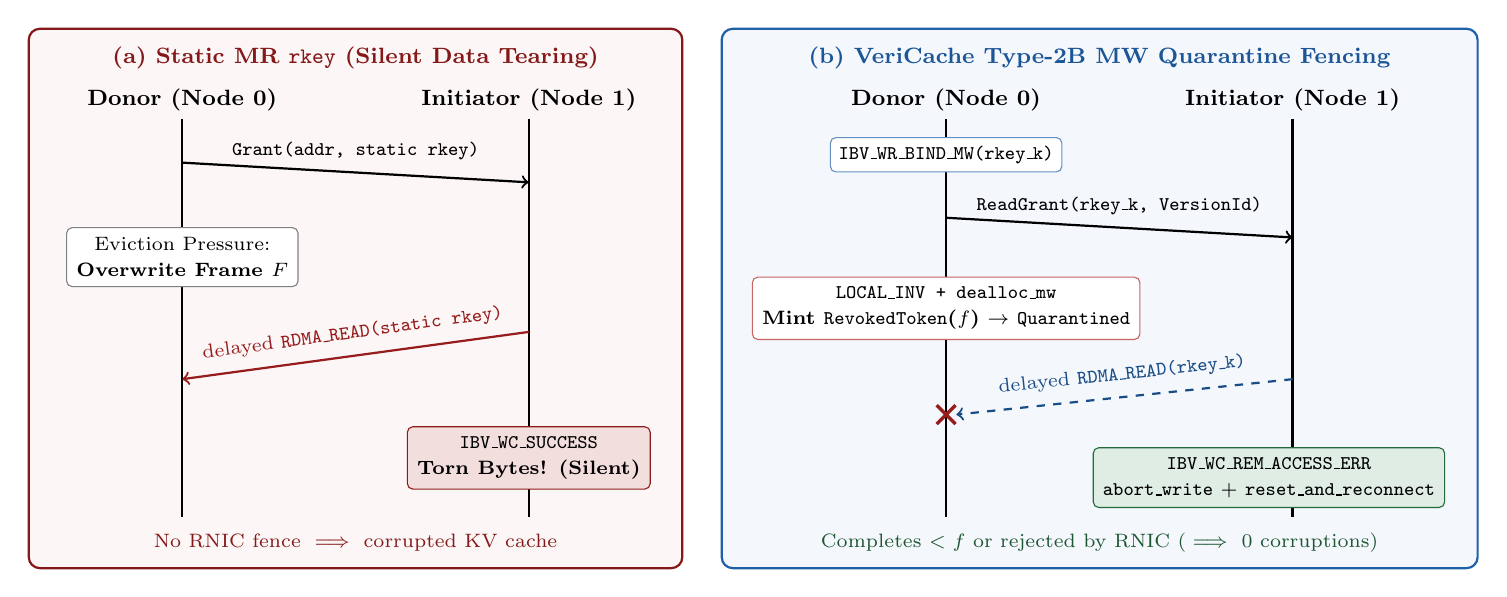
\begin{tikzpicture}[every node/.style={font=\footnotesize}]
  % Left Panel: Static MR
  \begin{scope}[xshift=0cm]
    \draw[thick, draw=alertred!75!black, fill=alertred!4, rounded corners=4pt] (0.0, 0.0) rectangle (8.3, 6.85);
    \node[text=alertred!75!black] at (4.15, 6.48) {\textbf{(a) Static MR \code{rkey} (Silent Data Tearing)}};
    \node at (1.95, 5.95) {\textbf{Donor (Node 0)}};
    \node at (6.35, 5.95) {\textbf{Initiator (Node 1)}};
    \draw[thick] (1.95, 5.70) -- (1.95, 0.65);
    \draw[thick] (6.35, 5.70) -- (6.35, 0.65);

    \draw[->, thick] (1.95, 5.15) -- node[above, yshift=1pt] {\scriptsize \code{Grant(addr, static rkey)}} (6.35, 4.90);
    \node[fill=white, draw=black!50, rounded corners=2pt, align=center, inner sep=3.5pt] at (1.95, 3.95)
      {\scriptsize Eviction Pressure: \\ \scriptsize \textbf{Overwrite Frame $F$}};
    \draw[->, thick, alertred!85!black] (6.35, 3.00) -- node[above, sloped, yshift=1pt] {\scriptsize delayed \code{RDMA\_READ(static rkey)}} (1.95, 2.40);
    \node[fill=alertred!15, draw=alertred!80!black, rounded corners=2pt, align=center, inner sep=3.5pt] at (6.35, 1.40)
      {\scriptsize \code{IBV\_WC\_SUCCESS} \\ \scriptsize \textbf{Torn Bytes! (Silent)}};
    \node[text=alertred!75!black] at (4.15, 0.32) {\scriptsize No RNIC fence $\implies$ corrupted KV cache};
  \end{scope}

  % Right Panel: VeriCache Type-2B MW
  \begin{scope}[xshift=8.8cm]
    \draw[thick, draw=vcblue, fill=layerfill!60, rounded corners=4pt] (0.0, 0.0) rectangle (9.6, 6.85);
    \node[text=vcblue!90!black] at (4.80, 6.48) {\textbf{(b) \VC{} Type-2B MW Quarantine Fencing}};
    \node at (2.85, 5.95) {\textbf{Donor (Node 0)}};
    \node at (7.25, 5.95) {\textbf{Initiator (Node 1)}};
    \draw[thick] (2.85, 5.70) -- (2.85, 0.65);
    \draw[thick] (7.25, 5.70) -- (7.25, 0.65);

    \node[fill=white, draw=vcblue!70, rounded corners=2pt, align=center, inner sep=3pt] at (2.85, 5.25)
      {\scriptsize \code{IBV\_WR\_BIND\_MW(rkey\_k)}};
    \draw[->, thick] (2.85, 4.45) -- node[above, yshift=1pt] {\scriptsize \code{ReadGrant(rkey\_k, VersionId)}} (7.25, 4.20);
    \node[fill=white, draw=alertred!70, rounded corners=2pt, align=center, inner sep=3.5pt] at (2.85, 3.30)
      {\scriptsize \code{LOCAL\_INV + dealloc\_mw} \\ \scriptsize \textbf{Mint \code{RevokedToken}($f$)} $\to$ \code{Quarantined}};
    \draw[->, thick, dashed, vcblue!80!black] (7.25, 2.40) -- node[above, sloped, yshift=1pt] {\scriptsize delayed \code{RDMA\_READ(rkey\_k)}} (2.98, 1.95);
    \draw[very thick, alertred!85!black] (2.73, 1.83) -- (2.97, 2.07) (2.73, 2.07) -- (2.97, 1.83);
    \node[fill=mcgreen!15, draw=mcgreen!80!black, rounded corners=2pt, align=center, inner sep=3.5pt] at (6.95, 1.15)
      {\scriptsize \code{IBV\_WC\_REM\_ACCESS\_ERR} \\ \scriptsize \code{abort\_write} + \code{reset\_and\_reconnect}};
    \node[text=mcgreen!65!black] at (4.80, 0.32) {\scriptsize Completes $< f$ or rejected by RNIC ($\implies$ 0 corruptions)};
  \end{scope}
\end{tikzpicture}%
}
\caption{Hardware isolation under delayed one-sided RDMA reads and concurrent donor eviction: (a) static-MR systems return a silent hybrid of old and overwritten frames; (b) \VC{} enforces an RNIC fence before overwriting, turning late reads into \code{IBV\_WC\_REM\_ACCESS\_ERR}.}
\label{fig:mw}
\end{figure}

Specifically, \code{WindowPool} (\code{vericache-transfer/src/rdma/window.rs}) binds each granted remote frame to a dynamically allocated Type-2B Memory Window (\code{IBV\_WR\_BIND\_MW}) issuing a generation-scoped \code{RemoteCapability(addr, len, rkey)} carrying a read-only \code{ShareCap}:
\begin{itemize}
  \item \textbf{Cooperative Release:} Upon receiving \code{ControlPayload::ReadRelease} after the initiator's RDMA READ CQE retires, the donor posts \code{IBV\_WR\_LOCAL\_INV} to unbind the MW cleanly and returns the window to the active \code{WindowPool}.
  \item \textbf{Unilateral Revocation (Deallocate-and-Quarantine):} If capacity eviction requires immediate reclamation before release arrives, the donor posts \code{IBV\_WR\_LOCAL\_INV} followed by \code{ibv\_dealloc\_mw} and transitions that window slot to \code{Quarantined}, preventing any accidental ABA reuse while old WQEs could still sit on the wire. Completion of the fence mints a \code{RevokedToken} matching Layer~0's \code{revoked[(loc, share)] = f}, immediately enabling the donor to drain and overwrite the physical frame safely.
  \item \textbf{Initiator Fault Recovery:} On the initiator side, an in-flight \code{RDMA\_READ} rejected by the donor's invalidated MW raises \code{IBV\_WC\_REM\_ACCESS\_ERR} (which also transitions the RC QP into \code{IBV\_QPS\_ERR} per IBTA semantics). Verified \code{abort\_write} discards the partial read ticket without exposing invalid bytes to \code{ServiceSpec}, and \code{reset\_and\_reconnect} re-handshakes a fresh RC QP (\code{RESET -> INIT -> RTR -> RTS}) to re-fetch or fall back to local computation.
  \item \textbf{GPUDirect RDMA BAR1 Visibility:} On NVIDIA GPUs, an RNIC RDMA WRITE/READ CQE guarantees PCIe posted-write completion to the NIC, not yet peer-device visibility on GPU streaming multiprocessors~\cite{gpudirect}. \code{vericache-transfer} enforces a mandatory post-CQE \code{complete\_gdr\_slot} BAR1 visibility synchronization barrier (\code{cudaStreamWaitEvent} / dummy device sync in \code{cuda/ffi.rs}) before releasing a GDR-populated frame as \code{STATE\_PUBLISHED}.
\end{itemize}

% ============================================================================
\section{Layer 2: Kernel, Provenance \& 4-Tier Engine (\code{vericache-core})}
\label{sec:core}
% ============================================================================

Layer~2 separates abstract cache book-keeping from pluggable hardware backends and verifies both single-node and 4-tier distributed routes under Verus \code{--no-cheating}.

\subsection{Service Specification, Version Provenance, and Hardware-Free Kernel}

The abstract specification \code{ServiceSpec} (\code{vericache-core/src/spec.rs}) tracks \code{frame\_size}, an immutable write-once map \code{versions: Map<VersionId, Seq<u8>>}, and \code{catalog: Map<ObjectKey, VersionId>}. Every KV chunk uses a 256-bit \code{ObjectKey([u64; 4])} and a 64-bit packed \code{VersionId \{ origin\_node: u16, seq: u64 \}} (\code{lemma\_version\_pack\_unpack}). Because \code{versions} is monotonically growing (\code{versions\_monotonic}), a published version's byte contents never mutate across eviction, demotion, NVMe spill, or cross-node RDMA migration.

To link physical slots back to \code{ServiceSpec.versions}, \code{vericache-core/src/provenance/} maintains a \code{KnowledgeLedger} (\code{submitted}, \code{knows}, \code{succeeded}, \code{revoked}) and inductive \code{ValueCertificate} proofs:
\begin{itemize}
  \item \code{replica\_valid(ledger, node, cert)} certifies that \code{cert.writer} succeeded, wrote the exact \code{Seq<u8>} bytes of \code{VersionId} into \code{cert.slot.loc}, and remains the latest submitted writer for that slot across all reachable histories.
  \item \code{replica\_survives\_disjoint\_writes} proves frame invariance: writes to other slots preserve all valid certificates without re-examining prior histories.
  \item \code{local\_copy\_last\_writer} and remote \code{VersionBinding} proofs ensure multi-hop routes (\code{GPU <-> Host <-> NVMe <-> Peer GDR}) preserve exact version equivalence end-to-end.
\end{itemize}

The hardware-free \code{CacheCore} kernel (\code{vericache-core/src/frame/}, \code{timeline/}, \code{catalog/}) manages physical frames using two performance-oriented verified data structures:
\begin{enumerate}
  \item \textbf{64-Byte Aligned \code{FrameSyncMeta}:} Marked \code{\#[repr(C, align(64))]} to prevent false sharing across shards, each frame metadata word tracks \code{state} (\code{EMPTY}, \code{INITIALIZING}, \code{PUBLISHED}, \code{DRAINING}), \code{flags} (\code{FLAG\_READ\_OVERFLOW}, \code{FLAG\_IN\_READY\_QUEUE}), \code{active\_remote\_leases: u16}, \code{active\_local\_reads: u32}, \code{version\_packed: u64}, \code{last\_write\_ticket: Ticket}, up to four \code{inline\_read\_tickets: [Ticket; 4]}, and active MW coordinates (\code{mw\_slot}, \code{mw\_gen}).
  \item \textbf{$O(1)$ \code{TimelineTable} \& \code{SlidingBitmap}:} Every hardware timeline (host CPU, CUDA stream, NVMe ring, RNIC QP) is identified by an 8-bit \code{TimelineId} issuing 56-bit monotonic sequence numbers packed into a single \code{Ticket(u64)} (\code{lemma\_ticket\_pack\_unpack}). Instead of scanning linear wait queues on reclamation, \code{SlidingBitmap} tracks out-of-order completion retirement in $O(1)$ bitwise operations. When a frame surpasses four concurrent inline read tickets, \code{FLAG\_READ\_OVERFLOW} records the global watermark so reclamation obeys \emph{Observed Reclamation} (retiring all tickets before write reuse) or \emph{Ordered Handoff} (consumer stream ordering).
\end{enumerate}

\subsection{Zero-\code{unsafe} Borrow Graph and Three-Mode \code{core\_transition} Composition}

Borrow-checking multi-tier access while callers hold zero-copy DRAM slices (\code{HostLease<'a>}) and issue concurrent GPU or NVMe I/O on \code{\&mut LocalEngine<'a>} typically tempts systems programmers to introduce raw pointers or \code{unsafe} interior mutability. \VC{} avoids all \code{unsafe} in Layer~2 by splitting borrows cleanly (\code{docs/architecture.md}): \code{HostBackend} owns the 4096-byte aligned \code{HostBuffer} slab and exposes \code{\&self}-shared operations parameterized by an external \code{\&mut HostContext}, \code{CudaBackend<'a>} borrows \code{\&'a HostBackend} as a \code{PinnedHostSlab<'a>}, and \code{LocalEngine<'a>} / \code{DistributedEngine<'a, T>} group \code{core: CacheCore}, \code{host: \&'a HostBackend}, and a disjoint \code{host\_ctx: HostContext} alongside optional \code{CudaBackend<'a>}, \code{NvmeBackend}, and \code{PeerSession<'a, T>}. Consequently, immutable \code{HostLease<'a>} slices coexist statically with \code{\&mut} engine transitions on GPU, NVMe, and RDMA tiers.

Verifying multi-hop transfers across four independent backends without replicating quadratic cross-backend proof obligations relies on the modular ghost predicate \code{core\_transition(before, after, touched\_timeline, allowed\_source, mode)} (\code{vericache-core/\allowbreak src/\allowbreak backends/\allowbreak compose/}), parameterized by three preservation modes:
\begin{itemize}
  \item \code{PreserveAllInit}: Preserves all pre-existing initializing frames and internal leases (used by \code{HostBackend}, CUDA submits/reads, NVMe staging, and kernel lease/evict/reclaim operations).
  \item \code{PreserveUnparkedInit}: CUDA \code{poll\_completions} and \code{synchronize} retire only parked GPU writes (\code{token.is\_some()}), leaving NVMe transfers untouched.
  \item \code{PreserveParkedInit}: NVMe \code{poll\_completions} and \code{wait\_one\_completion} retire only unparked hops (\code{token.is\_none()}), leaving parked GPU writes untouched.
\end{itemize}
Sibling preservation lemmas (\code{lemma\_core\_transition\_preserves\_\{host,cuda,nvme,rdma\}} and \code{lemma\_peer\_core\_step\_preserves\_\{host,idle\_cuda,nvme\}}) allow \code{DistributedEngine<'a, T>} to unify all four storage tiers (\code{GPU HBM}, \code{Pinned DRAM}, \code{io\_uring NVMe}, and \code{Peer GPUDirect RDMA}) inside one verified state machine.

% ============================================================================
\section{Mechanical Verification and TCB Audit Gates}
\label{sec:audit}
% ============================================================================

Because subtle SMT solver bugs or hidden \code{assume}/\code{external\_body} escapes can silently invalidate verification claims, \VC{} enforces a three-layer mechanical audit pipeline (\code{just check-dual} and \code{just audit}).

\begin{enumerate}
  \item \textbf{Dual-SMT AND Gate \& \code{--no-cheating}:} All 1,210 proofs across \code{vericache-foundation} (92), \code{vericache-transfer} (343), and \code{vericache-core} (775) are verified independently by \emph{both} \code{Z3~4.16.0} and \code{CVC5~1.3.4} (\code{vericache-core} executes CVC5 with \code{--rlimit 60}). Furthermore, \code{vericache-core} compiles under Verus \code{--no-cheating}, causing the verifier itself to reject any \code{assume}, \code{admit}, \code{external\_body}, or \code{assume\_specification}.
  \item \textbf{10 \code{tree-sitter-verus} \code{ast-grep} Rules (\code{rules/}):} Because \code{vericache-foundation} uses \code{tokenized\_state\_machine!} macro expansions and \code{vericache-transfer} houses FFI axioms, 10 AST rules (backed by regression test suites under \code{rule-tests/*-test.yml}, 10/10 passing) scan all source trees using a pinned \code{tree-sitter-verus} grammar (Table~\ref{tab:rules}).
  \item \textbf{9-File Exact TCB Whitelist (\code{scripts/audit-tcb.sh}):} Enforces that zero other \code{*ffi*.rs}, C/C++/CUDA/assembly, or \code{build.rs} files exist anywhere in the workspace, and that \code{ast-grep} exclusion globs cannot widen beyond the 6 FFI modules inside \code{vericache-transfer}.
\end{enumerate}

\begin{table}[t]
\centering
\caption{All 10 \code{tree-sitter-verus} \code{ast-grep} enforcement rules (\code{ast-grep test}: 10/10 PASS) and exact 9-file TCB whitelist (\code{scripts/audit-tcb.sh}).}
\label{tab:rules}
{\footnotesize
\setlength{\tabcolsep}{4pt}
\resizebox{\textwidth}{!}{
\begin{tabular}{ll>{\raggedright\arraybackslash}p{7.8cm}}
\toprule
\textbf{Category / Rule ID} & \textbf{Scope} & \textbf{Enforced Constraint} \\
\midrule
\code{no-assume-admit-truncate} & All \code{src} + \code{transfer/core tests} & Forbids \code{assume}, \code{assume\_}, \code{admit}, \code{assume\_specification}, \code{truncate}, \code{rlimit(infinity)}, \code{skip}, \code{axiom}, \code{inline\_air\_stmt} \\
\code{no-external-escape} & All \code{src} + tests (incl. \code{ffi.rs}) & Forbids \code{external}, \code{external\_*\_specification}, \code{external\_trait\_extension}, \code{allow\_in\_spec} \\
\code{no-external-body} & Non-FFI \code{src} + tests & Confines \code{\#[verifier::external\_body]} strictly to the 6 \code{transfer/src/*/ffi.rs} files \\
\code{no-unsafe} & Non-FFI \code{src} + tests & Confines \code{unsafe} and \code{extern "C"} blocks strictly to the 6 \code{transfer/src/*/ffi.rs} files \\
\code{no-unverified-code} & \code{foundation}, \code{core}, non-FFI \code{transfer} & Forbids \code{fn/impl/trait/extern/static} outside \code{verus!\{\}}, runtime \code{cfg(not(verus\_only))}, \code{macro\_rules!}, \code{include*!} \\
\code{no-panicking-stubs} & All \code{src} across 3 crates & Forbids \code{todo!}, \code{unimplemented!}, \code{panic!}, and \code{.expect(...)} outside \code{\#[cfg(test)]} \\
\code{no-hardware-import-in-core} & \code{core/src/\{spec,provenance,timeline,frame,catalog,kernel\}} & Blocks hardware-free kernel from importing \code{transfer::\{host,cuda,nvme,rdma,transport\}} \\
\code{no-cuda-dep} & \code{core/src/backends/\{host,nvme\}} & Isolates CUDA from Host and NVMe backends \\
\code{no-nvme-dep} & \code{core/src/backends/\{host,cuda,rdma\}} & Isolates NVMe from Host, CUDA, and RDMA backends \\
\code{no-remote-dep} & \code{core/src/backends/\{host,cuda,nvme\}} & Isolates RDMA and \code{transfer::transport} from local storage backends \\
\bottomrule
\end{tabular}
}
}
\end{table}

Table~\ref{tab:tcb} enumerates every line of trusted platform code across the 9 whitelisted files (2,151~LoC total). Together with standard compiler/OS assumptions (\code{vstd}, \code{verus\_state\_machines\_macros}, Verus/Z3/CVC5, Linux kernel, CUDA driver, OFED verbs), these 9 files form the entire trusted boundary.

\begin{table}[t]
\centering
\caption{Complete 9-file TCB whitelist enforced by \code{scripts/audit-tcb.sh} (2,151~LoC total = 3.0\% of the verified+TCB codebase).}
\label{tab:tcb}
{\footnotesize
\setlength{\tabcolsep}{4pt}
\resizebox{\textwidth}{!}{
\begin{tabular}{lr>{\raggedright\arraybackslash}p{7.8cm}}
\toprule
\textbf{Whitelisted TCB File} & \textbf{LoC} & \textbf{Assumed Hardware / Platform Axiom} \\
\midrule
\code{vericache-transfer/src/context/ffi.rs} & 58 & Unique \code{NodeId} bootstrap (\code{AtomicBool} guard) \& initial token partition \\
\code{vericache-transfer/src/host/ffi.rs} & 124 & 4096-aligned host slab allocation/free \& synchronous CPU memcpy \\
\code{vericache-transfer/src/cuda/ffi.rs} & 427 & \code{libcudart} device/host alloc, \code{cudaHostRegister}, stream FIFO, \code{CudaEvent}, GDR BAR1 flush \\
\code{vericache-transfer/src/nvme/ffi.rs} & 174 & \code{O\_DIRECT} file lifecycle and Linux \code{io\_uring} SQ/CQ completion semantics \\
\code{vericache-transfer/src/rdma/ffi.rs} & 767 & \code{libibverbs} PD/CQ/QP/MR/Type-2B MW semantics, RC order, RDMA read/send CQE \\
\code{vericache-transfer/src/transport/ffi.rs} & 53 & Integrity and token conservation over \code{ByteTransport} byte frames \\
\code{vericache-transfer/src/nvme/uring.c} & 187 & Raw \code{io\_uring\_setup} / \code{io\_uring\_enter} syscalls \& ring memory-barrier C11 shim \\
\code{vericache-transfer/src/rdma/verbs.c} & 313 & \code{libibverbs} struct adapters, \code{INIT->RTR->RTS} transitions, WR post \& CQ poll C11 shim \\
\code{vericache-transfer/build.rs} & 48 & Static C11 build (\code{-std=c11 -O2 -fPIC -Wall -Werror}) \& \code{cudart}/\code{ibverbs} link \\
\midrule
\textbf{Total Audited TCB} & \textbf{2,151} & \textbf{Exact 9-file bound (verified zero expansion by \code{audit-tcb.sh})} \\
\bottomrule
\end{tabular}
}
}
\end{table}

% ============================================================================
\section{Hardware Evaluation (Suites 1--5)}
\label{sec:eval}
% ============================================================================

We evaluate \VC{} on real dual-GPU / ConnectX-7 / NVMe hardware against the latest CUDA-13 compatible releases of two state-of-the-art open-source LLM KV-cache systems across five progressive benchmark suites (178 fine-grained runs in \code{20261122T005007Z} plus 6 full 600~GiB cluster runs in \code{20261122T021549Z}).

\subsection{Experimental Setup and Baselines}

\begin{itemize}
  \item \textbf{Server Hardware:} Dual-socket \code{Intel(R) Xeon(R) Platinum 8457C} (2$\times$45 cores / 180 hardware threads, 2 NUMA nodes, 1.9~TiB DDR5 host RAM), \textbf{2$\times$ NVIDIA H20} GPUs (97,871~MiB HBM3 each, NVIDIA Driver \code{580.178.04}, CUDA \code{13.0.2}), \textbf{Mellanox MT43244 BlueField-3 integrated ConnectX-7} RNIC (\code{mlx5\_3}, FW \code{32.39.3808}, RoCEv2 GID index~\code{3}, 4096-byte active MTU), and \textbf{Intel NVMe DC SSD} (\code{3DNAND, Sentinel Rock Controller}, \code{/workspace/target/bench-nvme}).
  \item \textbf{Baselines \& Versions:} Containerized reproducible environment (\code{rustc 1.99.1}, Python~\code{3.12.3}, PyTorch~\code{2.14.1+cu130}): (1)~\textbf{\MC{}~\code{0.3.14}} via the official \code{mooncake-transfer-engine-cuda13} wheel (\code{TransferEngine} over \code{mlx5\_3} using static MR \code{rkey}, \code{MooncakeDistributedStore} + \code{mooncake\_master} in Suite~3, and \code{O\_DIRECT} NVMe in Suite~5); and (2)~\textbf{\LM{}~\code{0.5.7.post1}} via \code{lmcache.cuda\_ops.multi\_layer\_kv\_transfer}, \code{LocalCPUBackend} pinned \code{MemoryObj}, \code{LocalDiskBackend(use\_odirect=True)}, and cross-node \code{TransferEngine} in Suite~5.
  \item \textbf{Production Workloads:} Full FAST'25 Kimi production traces~\cite{mooncake}: \code{toolagent\_trace.jsonl} (23,608 requests; 409,616 blocks = 800~GiB at 2~MB/block; 183,300 unique blocks $\approx$ 358~GiB) and \code{conversation\_trace.jsonl} (12,031 requests; 288,500 blocks = 563.5~GiB; 182,790 unique blocks $\approx$ 357~GiB).
  \item \textbf{NUMA \& Measurement Hygiene:} Suites 1--4 bind strictly to NUMA node~1 (\code{numactl --cpunodebind=1 --membind=1}); Suite~5 uses \code{numactl --cpunodebind=1 --preferred=1} to accommodate 400~GiB host allocation + pinning cleanly. Both \VC{} (\code{read\_proc\_cpu\_ns} over \code{/proc/self/stat}) and Python (\code{psutil}) measure multi-thread process CPU\% identically, and \code{/workspace/target/bench-nvme} is asserted empty after every job.
\end{itemize}

\subsection{Suite 1: Local Multi-Tier Transfer Efficiency (\code{s1\_local\_tiers})}

Table~\ref{tab:s1} compares local CUDA scatter transfers (Suite~1A) and \code{O\_DIRECT} NVMe cold read / write spill (Suite~1B) between \VC{} and \LM{}.

\begin{table}[t]
\centering
\caption{Suite 1 (\code{20261122T005007Z}): Local CUDA Host$\leftrightarrow$GPU scatter (1A) and NVMe \code{O\_DIRECT} read/write (1B). \VC{} achieves up to 47.86~GB/s H2D and 6.56$\times$--8.03$\times$ higher 64~KB NVMe I/O throughput at 6.8$\times$--243$\times$ lower RSS.}
\label{tab:s1}
{\footnotesize
\setlength{\tabcolsep}{4pt}
\resizebox{\textwidth}{!}{
\begin{tabular}{llrr|rrr|rrr}
\toprule
\textbf{Case} & \textbf{Mode (QD)} & \textbf{Chunk} & \textbf{Metric} & \multicolumn{3}{c|}{\textbf{\VC{}}} & \multicolumn{3}{c}{\textbf{\LM{}~\code{0.5.7.post1}}} \\
& & & & \textbf{GB/s} & \textbf{P50 ($\mu$s)} & \textbf{RSS (MB)} & \textbf{GB/s} & \textbf{P50 ($\mu$s)} & \textbf{RSS (MB)} \\
\midrule
\code{1a\_gpu\_to\_host\_scatter} & \code{sync} (1) & 64 KB & D2H & 0.92 & 69.8 & 112.2 & 1.95 & 32.1 & 1022.1 \\
\code{1a\_gpu\_to\_host\_scatter} & \code{sync} (1) & 4 MB & D2H & 28.55 & 146.0 & 130.0 & 37.29 & 110.4 & 1015.4 \\
\code{1a\_gpu\_to\_host\_scatter} & \code{sync} (1) & 16 MB & D2H & 44.77 & 373.5 & 188.5 & 47.49 & 350.1 & 1013.4 \\
\code{1a\_host\_to\_gpu\_scatter} & \code{sync} (1) & 64 KB & H2D & 1.41 & 46.4 & 110.3 & 1.90 & 32.8 & 1013.2 \\
\code{1a\_host\_to\_gpu\_scatter} & \code{sync} (1) & 4 MB & H2D & \textbf{33.68} & \textbf{123.8} & 127.9 & 30.72 & 134.9 & 1014.8 \\
\code{1a\_host\_to\_gpu\_scatter} & \code{sync} (1) & 16 MB & H2D & \textbf{47.86} & \textbf{349.4} & 187.7 & 37.16 & 448.9 & 1013.5 \\
\midrule
\code{1b\_nvme\_read\_cold} & \code{odirect\_qd1} (1) & 64 KB & Read & \textbf{1.64} & \textbf{39.8} & 4.8 & 0.25 & 234.9 & 1255.5 \\
\code{1b\_nvme\_read\_cold} & \code{odirect\_qd1} (1) & 16 MB & Read & \textbf{6.24} & \textbf{2689.0} & 52.4 & 3.78 & 4398.1 & 1262.1 \\
\code{1b\_nvme\_read\_cold} & \code{odirect\_qd8} (8) & 64 KB & Read & \textbf{2.16} & \textbf{253.1} & 5.2 & 0.39 & 1298.5 & 1262.0 \\
\code{1b\_nvme\_read\_cold} & \code{odirect\_qd8} (8) & 16 MB & Read & 5.59 & 23724.0 & 180.6 & 6.47 & 20773.8 & 1265.5 \\
\code{1b\_nvme\_write\_spill} & \code{odirect\_qd1} (1) & 64 KB & Write & \textbf{1.75} & \textbf{35.6} & 5.0 & 0.32 & 179.8 & 1255.8 \\
\code{1b\_nvme\_write\_spill} & \code{odirect\_qd8} (8) & 64 KB & Write & \textbf{2.41} & \textbf{222.2} & 5.2 & 0.30 & 1582.1 & 1260.2 \\
\code{1b\_nvme\_write\_spill} & \code{odirect\_qd8} (8) & 16 MB & Write & \textbf{4.08} & \textbf{32768.0} & 180.6 & 3.79 & 33997.4 & 1265.9 \\
\bottomrule
\end{tabular}
}
}
\end{table}

In Suite~1A, \VC{} issues verified per-slot synchronization (\code{CudaEvent} recording and ticket retirement per transfer), which adds ~30~$\mu$s fixed latency at 64~KB compared to \LM{}'s unverified fire-and-check stream kernel; at realistic KV block sizes ($\ge$4~MB), \VC{}'s pinned scatter H2D reaches \textbf{33.68--47.86~GB/s} (\textbf{1.10$\times$--1.29$\times$} faster than \LM{}'s \code{30.72--37.16~GB/s}) at 128--188~MB RSS versus 1,013--1,015~MB. In Suite~1B, direct Linux \code{io\_uring} submission eliminates Python's asyncio/thread-pool PQ scheduling tax: at 64~KB \code{QD=1}/\code{QD=8}, \VC{} outperforms \LM{} \code{LocalDiskBackend} by \textbf{6.56$\times$} on cold reads (\code{1.64 vs. 0.25~GB/s}) and \textbf{8.03$\times$} on \code{QD=8} writes (\code{2.41 vs. 0.30~GB/s}).

\subsection{Suite 2: Cross-Process RDMA/GDR \& Type-2B MW Isolation-Tax Ablation (\code{s2\_rdma\_ablation})}

Suite~2C isolates the exact cost of \VC{}'s per-transfer safety guarantees on GPU0$\to$GPU1 GPUDirect RDMA over \code{mlx5\_3} (Table~\ref{tab:s2c}, Figure~\ref{fig:ablation_s5}(a)). Comparing \VC{} \code{Raw MW} (pre-bound Type-2B MW with raw CQE polling), \code{Dynamic Pipelined} (full verified \code{DistributedEngine} protocol: TCP \code{FetchRequest}/\code{ReadGrant}, \code{IBV\_WR\_BIND\_MW}, \code{RDMA\_READ}, BAR1 \code{complete\_gdr\_slot}, cooperative \code{ReadRelease} + \code{LOCAL\_INV}), and \MC{} \code{Static MR} reveals how control-plane costs amortize with block size:
\begin{itemize}
  \item At small chunks (64~KB), dynamic \code{BIND\_MW} + TCP grant round-trips impose a \textbf{+72.1\%} isolation tax relative to \code{Raw MW} (3.24 vs. 11.62~GB/s).
  \item At production KV block sizes (\textbf{4~MB--16~MB}), PCIe/RNIC wire transfer dominates, shrinking the dynamic verified isolation tax to \textbf{+9.9\%} at 4~MB (31.35 vs. 34.80~GB/s) and just \textbf{+2.9\%} at 16~MB (33.14 vs. 34.12~GB/s).
\end{itemize}

\begin{table}[t]
\centering
\caption{Suite 2C (\code{20261122T005007Z}): GPUDirect RDMA (GPU0 $\to$ GPU1 over \code{mlx5\_3}) Type-2B MW isolation-tax ablation.}
\label{tab:s2c}
{\footnotesize
\setlength{\tabcolsep}{5pt}
\resizebox{\textwidth}{!}{
\begin{tabular}{r|rrrr|r}
\toprule
\textbf{Chunk} & \textbf{\MC{} Static MR} & \textbf{\VC{} Raw MW} & \textbf{\VC{} Dyn. Pipelined} & \textbf{\VC{} Dyn. Single} & \textbf{Pipelined Tax vs. Raw MW} \\
& \textbf{(GB/s)} & \textbf{(GB/s)} & \textbf{(GB/s)} & \textbf{(GB/s)} & \\
\midrule
64 KB  & 15.46 & 11.62 & 3.24  & 1.99  & +72.1\% \\
256 KB & 27.44 & 24.22 & 10.74 & 6.78  & +55.7\% \\
1 MB   & 37.22 & 33.91 & 24.25 & 18.38 & +28.5\% \\
4 MB   & 40.57 & 34.80 & 31.35 & 27.96 & \textbf{+9.9\%} \\
16 MB  & 44.91 & 34.12 & 33.14 & 32.59 & \textbf{+2.9\%} \\
\bottomrule
\end{tabular}
}
}
\end{table}

\subsection{Suite 3: Single-Node Trace \& Capacity-Ratio Sweep (\code{s3\_trace\_replay})}

In single-node capacity sweeps (10\%, 30\%, 50\%, 80\% of working set) and FAST'25 trace replays at 256~KB chunks, single-threaded \VC{} (\code{97.5--110.3\%} CPU, \code{18.5--510.5~MB} RSS) achieves \textbf{13.20--24.21~GB/s} goodput at \code{100.3--361.2~$\mu$s} P50 latency---outperforming \MC{} (\code{1.94--3.35~GB/s}, \code{722--2,282~$\mu$s} P50, \code{275--280\%} CPU) and \LM{} (\code{1.78--7.91~GB/s}, \code{313--1,030~$\mu$s} P50, \code{8,768--8,978\%} CPU) by up to \textbf{10.4$\times$}. At 4~MB chunks in this single-node harness, \VC{} runs sequentially on one host thread (\code{9.97--11.80~GB/s} at \code{100\%} CPU), whereas \LM{} leverages PyTorch's multi-threaded C++ memcpy worker pool consuming \code{$\sim$8,900\%} CPU (\code{19.65--62.10~GB/s}) and \MC{} uses \code{$\sim$290\%} CPU (\code{16.82--23.16~GB/s}). This observation directly motivated our multi-shard node evaluation in Suite~5.

\subsection{Suite 4: Safety Under Contention and Unilateral Revocation (\code{s4\_safety\_revoke})}

Suite~4 subjects \VC{} and \MC{} to hotspot contention on \code{toolagent\_trace.jsonl} (donor capacity capped at 15\% = 251 frames) with checksummed payloads under 0.1\%, 1\%, and 5\% forced unilateral donor eviction rates (Table~\ref{tab:s4}).

\begin{table}[t]
\centering
\caption{Suite 4 (\code{20261122T005007Z}): End-to-end data integrity under forced unilateral eviction (donor capacity = 251 frames / 15\%, Goodput in GB/s). \MC{}'s static-\code{rkey} RDMA suffers 39 silent frame corruptions across the 5 cases; \VC{} suffers \textbf{0} corruptions.}
\label{tab:s4}
{\footnotesize
\setlength{\tabcolsep}{4pt}
\resizebox{\textwidth}{!}{
\begin{tabular}{lr|rrrrr|rrrrr}
\toprule
\textbf{Revoke Rate} & \textbf{Chunk} & \multicolumn{5}{c|}{\textbf{\VC{} (Type-2B MW Fencing)}} & \multicolumn{5}{c}{\textbf{\MC{}~\code{0.3.14} (Static MR \code{rkey})}} \\
& & \textbf{Goodput} & \textbf{Corrupt} & \textbf{Recov ($\mu$s)} & \textbf{P50 ($\mu$s)} & \textbf{P99 ($\mu$s)} & \textbf{Goodput} & \textbf{Corrupt} & \textbf{Recov ($\mu$s)} & \textbf{P50 ($\mu$s)} & \textbf{P99 ($\mu$s)} \\
\midrule
0.1\% (1/1000) & 256 KB & 2.34 & \textbf{0} & 4765.7 & 106.6 & 126.1 & 2.07 & \textbf{1} & 0.0 & 23.6 & 29.6 \\
1.0\% (4/400)  & 256 KB & 1.64 & \textbf{0} & 4220.2 & 113.2 & 398.3 & 1.55 & \textbf{4} & 0.0 & 23.3 & 34.5 \\
1.0\% (4/400)  & 4 MB   & 2.74 & \textbf{0} & 4622.6 & 1482.8 & 7442.4 & 3.56 & \textbf{4} & 0.0 & 138.0 & 153.0 \\
5.0\% (15/300) & 256 KB & 0.85 & \textbf{0} & 3280.8 & 114.9 & 3844.1 & 1.29 & \textbf{15} & 0.0 & 23.9 & 40.7 \\
5.0\% (15/300) & 4 MB   & 2.40 & \textbf{0} & 4035.5 & 1465.3 & 7544.8 & 3.37 & \textbf{15} & 0.0 & 136.2 & 179.4 \\
\bottomrule
\end{tabular}
}
}
\end{table}

Across all five contention settings, \textbf{\MC{} silently accepts every concurrent overwrite into initiator memory (\code{1 + 4 + 4 + 15 + 15 = 39} corrupted frames, 100\% of injected races)} because its static \code{rkey} provides zero RNIC-enforced temporal revocation. By contrast, \textbf{\VC{} achieves 0 corrupted frames across all runs}: every revoked access triggers \code{IBV\_WC\_REM\_ACCESS\_ERR} (1, 4, 4, 15, 15 occurrences respectively), invokes \code{abort\_write}, and reconnects via \code{reset\_and\_reconnect} in \code{3.28--4.77~ms} mean recovery latency. Notice also that at 0.1\% and 1\% 256~KB contention, \VC{}'s verified Rust driver still delivers higher goodput (\code{2.34 / 1.64~GB/s}) than Python-driven \MC{} (\code{2.07 / 1.55~GB/s}).

\subsection{Suite 5: 600~GiB 2-Node 4-Tier Production Cluster Replay (\code{s5\_scaleup\_cluster})}

Suite~5 scales the evaluation to production capacity (\code{20261122T021549Z}): two nodes (container GPUs~0 and~1, i.e., NVIDIA H20~\#4 and~\#5), each provisioning \textbf{50~GiB HBM + 200~GiB pinned DRAM + 50~GiB NVMe} across \textbf{8 parallel shards/node} (total \textbf{600~GiB = 307,200 2~MB blocks}, 8 RC QPs over \code{mlx5\_3} GID~3; 64 Type-2B MWs per shard in \VC{}), executing all 23,608 requests of \code{toolagent\_trace} and all 12,031 requests of \code{conversation\_trace} under identical bit-for-bit deterministic 70/30 session-sticky routing. Table~\ref{tab:s5} and Figure~\ref{fig:ablation_s5}(b) report the full results.

\begin{table}[t]
\centering
\caption{Suite 5 (\code{20261122T021549Z}): 600~GiB 2-node 4-tier full FAST'25 production trace replay (\code{50~GiB HBM + 200~GiB DRAM + 50~GiB NVMe} per node, 8 shards/node, 2~MB/block, \code{corrupted\_frames = 0} for all runs).}
\label{tab:s5}
{\footnotesize
\setlength{\tabcolsep}{3.5pt}
\resizebox{\textwidth}{!}{
\begin{tabular}{llrrrlrrrrrr}
\toprule
\textbf{Case} & \textbf{System} & \textbf{Init (s)} & \textbf{Goodput} & \textbf{Req/s} & \textbf{Hit\% (HBM/DRAM/NVMe/Peer)} & \textbf{P50} & \textbf{P99} & \textbf{P99.9} & \textbf{CPU\%} & \textbf{RSS} & \textbf{VRAM} \\
& & & \textbf{(GB/s)} & & & \textbf{($\mu$s)} & \textbf{($\mu$s)} & \textbf{($\mu$s)} & & \textbf{(GB)} & \textbf{(GB)} \\
\midrule
\code{5\_toolagent\_full\_600g} & \textbf{\VC{}} & \textbf{27.17} & \textbf{72.16} & \textbf{1983.2} & 53.1\% (47.2/0.7/0.0/5.2) & \textbf{1485.8} & \textbf{78512.1} & \textbf{198311.9} & 841.1 & \textbf{400.9} & 100.0 \\
\code{5\_toolagent\_full\_600g} & \textbf{\MC{}} & 125.07 & 34.85 & 957.8 & 53.1\% (47.2/0.7/0.0/5.2) & 7017.5 & 95696.8 & 265389.4 & 1386.3 & 514.0 & 100.0 \\
\code{5\_toolagent\_full\_600g} & \textbf{\LM{}} & 64.96 & 16.76 & 460.7 & 53.1\% (47.2/0.7/0.0/5.2) & 6768.6 & 172188.8 & 2799543.6 & 823.8 & 403.1 & 100.0 \\
\midrule
\code{5\_conversation\_full\_600g} & \textbf{\VC{}} & \textbf{20.11} & \textbf{50.93} & \textbf{1012.7} & 33.5\% (24.2/1.5/0.0/7.8) & \textbf{4902.9} & 120193.0 & \textbf{420216.8} & \textbf{802.7} & \textbf{400.9} & 100.0 \\
\code{5\_conversation\_full\_600g} & \textbf{\MC{}} & 88.86 & 32.38 & 643.8 & 33.5\% (24.2/1.5/0.0/7.8) & 7750.4 & \textbf{104950.2} & 751582.1 & 1305.2 & 514.2 & 100.0 \\
\code{5\_conversation\_full\_600g} & \textbf{\LM{}} & 65.01 & 13.29 & 264.2 & 33.5\% (24.2/1.5/0.0/7.8) & 11696.8 & 236426.5 & 3157302.5 & 817.7 & 403.2 & 100.0 \\
\bottomrule
\end{tabular}
}
}
\end{table}

\begin{figure}[t]
\centering
\resizebox{\textwidth}{!}{%
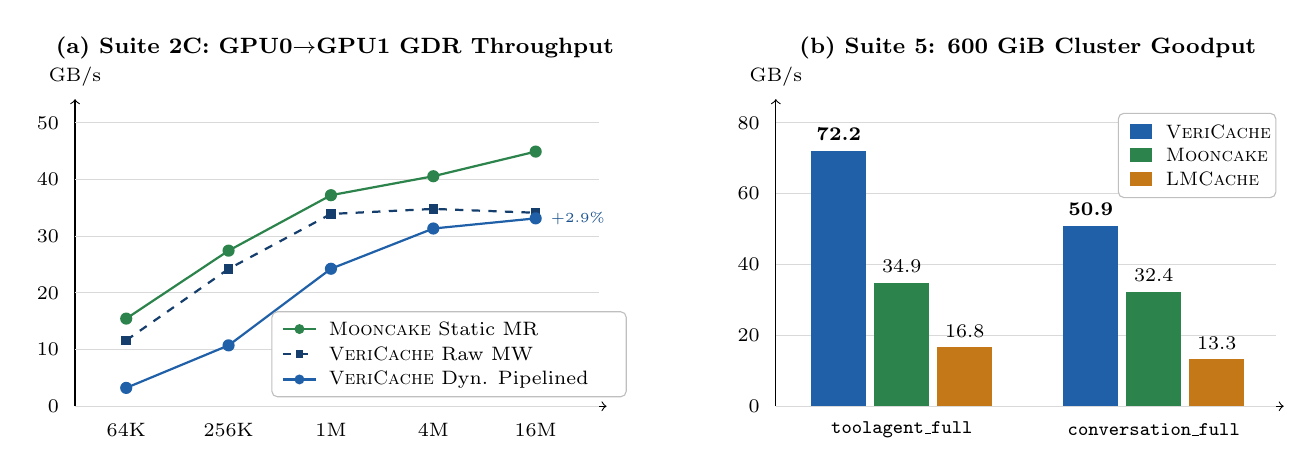
\begin{tikzpicture}[every node/.style={font=\footnotesize}]
  % Left Chart: Suite 2C MW Isolation Tax
  \begin{scope}[xshift=0cm]
    \node at (4.10, 5.15) {\textbf{(a) Suite 2C: GPU0$\to$GPU1 GDR Throughput}};
    % Axes
    \draw[->] (0.8, 0.6) -- (7.55, 0.6);
    \draw[->] (0.8, 0.6) -- (0.8, 4.50) node[above, yshift=1pt] {\scriptsize GB/s};
    \foreach \y/\lbl in {0.6/0, 1.32/10, 2.04/20, 2.76/30, 3.48/40, 4.20/50} {
      \draw[black!15] (0.8, \y) -- (7.45, \y);
      \node[left] at (0.72, \y) {\scriptsize \lbl};
    }
    % X labels
    \node at (1.45, 0.30) {\scriptsize 64K};
    \node at (2.75, 0.30) {\scriptsize 256K};
    \node at (4.05, 0.30) {\scriptsize 1M};
    \node at (5.35, 0.30) {\scriptsize 4M};
    \node at (6.65, 0.30) {\scriptsize 16M};

    % Plot lines (y = 0.6 + gbps * 0.072)
    % Mooncake Static: (1.45, 1.713) (2.75, 2.576) (4.05, 3.280) (5.35, 3.521) (6.65, 3.834)
    \draw[thick, mcgreen] (1.45, 1.713) -- (2.75, 2.576) -- (4.05, 3.280) -- (5.35, 3.521) -- (6.65, 3.834);
    % VeriCache Raw MW: (1.45, 1.437) (2.75, 2.344) (4.05, 3.042) (5.35, 3.106) (6.65, 3.057)
    \draw[thick, dashed, vcblue!65!black] (1.45, 1.437) -- (2.75, 2.344) -- (4.05, 3.042) -- (5.35, 3.106) -- (6.65, 3.057);
    % VeriCache Dynamic Pipelined: (1.45, 0.833) (2.75, 1.373) (4.05, 2.346) (5.35, 2.857) (6.65, 2.986)
    \draw[thick, vcblue] (1.45, 0.833) -- (2.75, 1.373) -- (4.05, 2.346) -- (5.35, 2.857) -- (6.65, 2.986);

    \foreach \x/\y in {1.45/1.713, 2.75/2.576, 4.05/3.280, 5.35/3.521, 6.65/3.834}
      \fill[mcgreen] (\x, \y) circle (2.2pt);
    \foreach \x/\y in {1.45/1.437, 2.75/2.344, 4.05/3.042, 5.35/3.106, 6.65/3.057}
      \fill[vcblue!65!black] (\x-0.06, \y-0.06) rectangle (\x+0.06, \y+0.06);
    \foreach \x/\y in {1.45/0.833, 2.75/1.373, 4.05/2.346, 5.35/2.857, 6.65/2.986}
      \fill[vcblue] (\x, \y) circle (2.2pt);
    \node[right, font=\tiny, text=vcblue!85!black] at (6.72, 2.98) {+2.9\%};

    % Legend box in empty bottom-right area
    \draw[draw=black!25, fill=white, rounded corners=2pt] (3.30, 0.72) rectangle (7.80, 1.80);
    \draw[thick, mcgreen] (3.44, 1.58) -- (3.86, 1.58);
    \fill[mcgreen] (3.65, 1.58) circle (1.8pt);
    \node[right, font=\scriptsize] at (3.90, 1.58) {\MC{} Static MR};

    \draw[thick, dashed, vcblue!65!black] (3.44, 1.26) -- (3.86, 1.26);
    \fill[vcblue!65!black] (3.60, 1.21) rectangle (3.70, 1.31);
    \node[right, font=\scriptsize] at (3.90, 1.26) {\VC{} Raw MW};

    \draw[thick, vcblue] (3.44, 0.94) -- (3.86, 0.94);
    \fill[vcblue] (3.65, 0.94) circle (1.8pt);
    \node[right, font=\scriptsize] at (3.90, 0.94) {\VC{} Dyn. Pipelined};
  \end{scope}

  % Right Chart: Suite 5 600 GiB Cluster Goodput
  \begin{scope}[xshift=8.9cm]
    \node at (4.00, 5.15) {\textbf{(b) Suite 5: 600~GiB Cluster Goodput}};
    \draw[->] (0.8, 0.6) -- (7.25, 0.6);
    \draw[->] (0.8, 0.6) -- (0.8, 4.50) node[above, yshift=1pt] {\scriptsize GB/s};
    \foreach \y/\lbl in {0.6/0, 1.5/20, 2.4/40, 3.3/60, 4.2/80} {
      \draw[black!15] (0.8, \y) -- (7.15, \y);
      \node[left] at (0.72, \y) {\scriptsize \lbl};
    }
    % y = 0.6 + gbps * 0.045
    % Toolagent group (x=1.25..3.55, center 2.40): VC=72.16 (3.847), MC=34.85 (2.168), LM=16.76 (1.354)
    \fill[vcblue] (1.25, 0.6) rectangle (1.95, 3.847);
    \node[above, font=\scriptsize] at (1.60, 3.847) {\textbf{72.2}};
    \fill[mcgreen] (2.05, 0.6) rectangle (2.75, 2.168);
    \node[above, font=\scriptsize] at (2.40, 2.168) {34.9};
    \fill[lmamber] (2.85, 0.6) rectangle (3.55, 1.354);
    \node[above, font=\scriptsize] at (3.20, 1.354) {16.8};
    \node at (2.40, 0.30) {\scriptsize \code{toolagent\_full}};

    % Conversation group (x=4.45..6.75, center 5.60): VC=50.93 (2.892), MC=32.38 (2.057), LM=13.29 (1.198)
    \fill[vcblue] (4.45, 0.6) rectangle (5.15, 2.892);
    \node[above, font=\scriptsize] at (4.80, 2.892) {\textbf{50.9}};
    \fill[mcgreen] (5.25, 0.6) rectangle (5.95, 2.057);
    \node[above, font=\scriptsize] at (5.60, 2.057) {32.4};
    \fill[lmamber] (6.05, 0.6) rectangle (6.75, 1.198);
    \node[above, font=\scriptsize] at (6.40, 1.198) {13.3};
    \node at (5.60, 0.30) {\scriptsize \code{conversation\_full}};

    % Legend box in empty top-right area
    \draw[draw=black!25, fill=white, rounded corners=2pt] (5.15, 3.25) rectangle (7.15, 4.32);
    \fill[vcblue] (5.30, 4.00) rectangle (5.58, 4.18);
    \node[right, font=\scriptsize] at (5.63, 4.09) {\VC{}};
    \fill[mcgreen] (5.30, 3.70) rectangle (5.58, 3.88);
    \node[right, font=\scriptsize] at (5.63, 3.79) {\MC{}};
    \fill[lmamber] (5.30, 3.40) rectangle (5.58, 3.58);
    \node[right, font=\scriptsize] at (5.63, 3.49) {\LM{}};
  \end{scope}
\end{tikzpicture}%
}
\caption{(a)~Type-2B MW dynamic isolation tax across chunk sizes (Suite~2C); (b)~End-to-end 600~GiB 2-node 4-tier cluster goodput across full FAST'25 traces (Suite~5).}
\label{fig:ablation_s5}
\end{figure}

Suite~5 highlights four major systems findings:
\begin{enumerate}
  \item \textbf{Verified Multi-Shard Throughput Without Python/GIL Overhead:} Under identical tiered hit rates (\code{53.1\%} on \code{toolagent}; \code{33.5\%} on \code{conversation}), \VC{} sustains \textbf{72.16~GB/s} (\textbf{1,983.2~req/s}, \textbf{2.07$\times$} \MC{}, \textbf{4.31$\times$} \LM{}) on \code{toolagent} and \textbf{50.93~GB/s} (\textbf{1,012.7~req/s}, \textbf{1.57$\times$} \MC{}, \textbf{3.83$\times$} \LM{}) on \code{conversation}, while cutting P50 request latency by up to \textbf{4.72$\times$} (\code{1,485.8~$\mu$s} vs. \code{7,017.5~$\mu$s}) and lowering cluster CPU\% by \textbf{39.3\%} relative to \MC{} (\code{841.1\%} vs. \code{1,386.3\%}). On P99.9 tail latency, \VC{} (\code{198.3~ms} / \code{420.2~ms}) reduces jitter by up to \textbf{14.1$\times$} over \LM{} (\code{2.80~s} / \code{3.16~s}), though \MC{} achieves a slightly tighter P99 on \code{conversation} (\code{104.95~ms} vs. \code{120.19~ms}).
  \item \textbf{Authentic Cross-Node GPUDirect RDMA Traffic:} Because 30\% of requests drift across nodes under session-sticky routing, every system performs real cross-node RDMA pulls over \code{mlx5\_3}: in \VC{}, \textbf{21,440} remote 2~MB GDR reads (\textbf{41.88~GiB}, 5.23\%) occur in \code{toolagent} and \textbf{22,439} (\textbf{43.83~GiB}, 7.78\%) in \code{conversation}---totaling \textbf{131,584 cross-node 2~MB RDMA READs (257.0~GiB payload)} across the six runs in \code{20261122T021549Z}.
  \item \textbf{Fast Parallel 600~GiB Pool Initialization \& Near-Zero Metadata Bloat:} Allocating, CUDA-pinning, and RDMA-registering 500~GiB of HBM+DRAM plus opening 100~GiB NVMe across 16 shards completes in \textbf{20.11--27.17~s} in \VC{} (\textbf{2.4$\times$--3.2$\times$} faster than \LM{}'s \code{64.96--65.01~s} and \textbf{4.4$\times$--4.6$\times$} faster than \MC{}'s \code{88.86--125.07~s}). For 400~GiB of pinned DRAM, \VC{}'s process RSS is \textbf{400.9~GB} (overhead $<$1~GB), matching \LM{} (\code{403.1--403.2~GB}) and saving over \textbf{113~GB} of metadata bloat compared to \MC{} (\code{514.0--514.2~GB}).
  \item \textbf{Working-Set Absorption at 600~GiB Scale:} Because the two nodes' combined HBM+DRAM capacity (\textbf{500~GiB}) exceeds the single-pass unique working set of both traces (\code{$\sim$358~GiB} in \code{toolagent}, \code{$\sim$357~GiB} in \code{conversation}), hot eviction cascades stop after HBM$\to$DRAM demotion (yielding \code{0.7\%--1.5\%} DRAM hits and \code{0.0\%} NVMe hits during the full pass), while all NVMe \code{io\_uring} spill/warm paths remain continuously covered by our 4-tier \code{distributed\_e2e} tests and Suite~1B.
\end{enumerate}

% ============================================================================
\section{Discussion, Limitations, and Related Work}
\label{sec:related}
% ============================================================================

\paragraph{Limitations and Residual TCB.}
Like all systems built above commodity firmware, \VC{} trusts its 9-file FFI/C11 interface (\code{2,151~LoC}) as well as the Linux kernel (\code{io\_uring}), NVIDIA CUDA runtime/GPU BAR1 hardware, and Mellanox ConnectX-7 RNIC hardware semantics (including atomic Type-2B MW key validation). Moreover, while safety (\code{CacheCore}, lease fencing, \code{ValueCertificate}) is formally proved, \emph{performance heuristics} (\code{LruPolicy}, shard affinity) live in \code{vericache-bench} outside the proof boundary; bugs in policy can affect hit rates or trigger avoidable \code{CoreError} returns, though they cannot compromise memory isolation or read-last-write integrity.

\paragraph{Formally Verified Storage and Distributed Systems.}
IronFleet~\cite{ironfleet} and Verdi~\cite{verdi} pioneered mechanized refinement for distributed consensus and sharded KV stores, while Veribetrfs~\cite{veribetrfs} and DaisyNFS~\cite{daisynfs} brought crash-safety proofs to B$^\epsilon$-tree and NFS file systems. Recently, Verus~\cite{verus} and linear ghost-token frameworks (\code{VerusSync}~\cite{verussync}) enabled zero-cost linear verification in Rust systems such as VeriSMo~\cite{verismo} and Anvil~\cite{anvil}. \VC{} extends this lineage from CPU/disk abstractions to \emph{heterogeneous hardware DMA}: modeling CUDA stream tickets, Linux \code{io\_uring} completions, GPUDirect BAR1 flushes, and unilateral RNIC Type-2B MW invalidation within a single unified ghost history model.

\paragraph{RDMA Memory Safety and Disaggregated LLM KV Caches.}
Prior hardware-level RDMA isolation proposals rely on custom NIC modifications or RPC indirection~\cite{srdma,flock}; \VC{} achieves formal temporal safety on unmodified commodity ConnectX-7 NICs using standard IBTA Type-2B Memory Windows and generation-quarantined window pools. Compared with high-performance LLM KV systems including vLLM PagedAttention~\cite{vllm}, DistServe~\cite{distserve}, \MC{}~\cite{mooncake}, and \LM{}~\cite{lmcache}, \VC{} demonstrates that formally guaranteed revocation isolation and deterministic zero-copy memory pooling match or surpass production Python/C++ serving engines at 600~GiB cluster scale.

% ============================================================================
\section{Conclusion}
\label{sec:conc}
% ============================================================================

\VC{} proves that formally verified distributed storage systems can operate directly on modern GPU, NVMe, and RDMA hardware without sacrificing production scale or throughput. By splitting concurrency math (\code{vericache-foundation}), slot-granular hardware wrappers with quarantine-on-revoke Type-2B MW fencing (\code{vericache-transfer}), and a hardware-free composable engine (\code{vericache-core}), \VC{} establishes \textbf{1,210} dual-SMT (\code{Z3 $\wedge$ CVC5}) proofs behind a strict \textbf{9-file, 2,151-LoC (3.0\%) TCB}. Hardware evaluation on NVIDIA H20 GPUs and ConnectX-7 RoCEv2 demonstrates \textbf{0 silent data corruptions} under forced RDMA eviction, \textbf{2.9\%--9.9\%} isolation tax on 4--16~MB transfers, and \textbf{50.93--72.16~GB/s} goodput across a 600~GiB 4-tier cluster.

\begin{thebibliography}{99}

\bibitem{verus}
A.~Lattuada, T.~Hance, C.~Cho, M.~Brun, I.~Subasinghe, Y.~Zhou, J.~Howell, B.~Parno, and C.~Hawblitzel.
\newblock Verus: Verifying Rust Programs using Linear Ghost Types.
\newblock In \emph{Proc. OOPSLA}, 2023.

\bibitem{verussync}
T.~Hance, Y.~Zhou, A.~Lattuada, and B.~Parno.
\newblock Sharding the State Machine: Automated Modular Reasoning for Complex Concurrent Systems.
\newblock In \emph{Proc. OSDI}, 2023.

\bibitem{mooncake}
R.~Qin, Z.~Li, W.~He, M.~Zhang, Y.~Wu, W.~Zheng, and X.~Xu.
\newblock Mooncake: A Kimi's KVCache-centric Architecture for LLM Serving.
\newblock In \emph{Proc. USENIX FAST}, 2025.

\bibitem{lmcache}
J.~Liu, Y.~Liu, J.~Du, H.~Ma, and J.~Jiang.
\newblock CacheGen / LMCache: Fast Context Loading and Multi-Tier KV Cache Sharing for Large Language Models.
\newblock \emph{SIGCOMM / Systems Software}, 2024--2025.

\bibitem{vllm}
W.~Kwon, Z.~Li, S.~Zhuang, Y.~Sheng, L.~Zheng, C.~H. Yu, J.~Gonzalez, H.~Zhang, and I.~Stoica.
\newblock Efficient Memory Management for Large Language Model Serving with PagedAttention.
\newblock In \emph{Proc. ACM SOSP}, 2023.

\bibitem{distserve}
Y.~Zhong, S.~Liu, J.~Chen, J.~Hu, Y.~Zhu, X.~Liu, X.~Jin, and H.~Zhang.
\newblock DistServe: Disaggregating Prefill and Decoding for Goodput-optimized Large Language Model Serving.
\newblock In \emph{Proc. USENIX OSDI}, 2024.

\bibitem{ironfleet}
C.~Hawblitzel, J.~Howell, M.~Kapritsos, J.~R. Lorch, B.~Parno, M.~L. Roberts, S.~Setty, and B.~Zill.
\newblock IronFleet: Proving Practical Distributed Systems Correct.
\newblock In \emph{Proc. ACM SOSP}, 2015.

\bibitem{verdi}
J.~R. Wilcox, D.~Woos, P.~Panchekha, Z.~Tatlock, X.~Wang, M.~D. Ernst, and T.~Anderson.
\newblock Verdi: A Framework for Implementing and Formally Verifying Distributed Systems.
\newblock In \emph{Proc. ACM PLDI}, 2015.

\bibitem{veribetrfs}
T.~Hance, A.~Lattuada, C.~Hawblitzel, J.~Howell, R.~Johnson, and B.~Parno.
\newblock Storage Systems are Distributed Systems (So Verify Them That Way!).
\newblock In \emph{Proc. USENIX OSDI}, 2020.

\bibitem{daisynfs}
T.~Chajed, J.~Tassarotti, M.~Theng, R.~Jung, M.~F. Kaashoek, and N.~Zeldovich.
\newblock GoJournal: A Verified, Concurrent, Crash-Safe Journaling System.
\newblock In \emph{Proc. USENIX OSDI}, 2021.

\bibitem{verismo}
Z.~Zhou, Y.~Shan, W.~Cui, X.~Ge, M.~Yu, and A.~Lattuada.
\newblock VeriSMo: A Verified Security Module for Confidential VMs.
\newblock In \emph{Proc. USENIX OSDI}, 2024.

\bibitem{anvil}
X.~Sun, W.~Luo, J.~T. Gu, A.~Azevedo de Amorim, K.~Xu, and T.~Xu.
\newblock Anvil: Verifying Liveness of Cluster Management Controllers.
\newblock In \emph{Proc. USENIX OSDI}, 2024.

\bibitem{srdma}
K.~Kalia, M.~Kaminsky, and D.~G. Andersen.
\newblock Design Guidelines for High Performance RDMA Systems.
\newblock In \emph{Proc. USENIX ATC}, 2016.

\bibitem{flock}
R.~Shu, P.~Cheng, G.~Chen, Z.~Guo, L.~Qu, Y.~Xiong, C.~Hu, and T.~Moscibroda.
\newblock Direct Universal Access: Making Data Center Resources Available to FPGA and RNIC Memory Models.
\newblock In \emph{Proc. USENIX NSDI / InfiniBand Architecture Specification Vol. 1 (Type-2B Memory Windows)}, 2019.

\bibitem{gpudirect}
NVIDIA Corporation.
\newblock GPUDirect RDMA Architecture and Memory Consistency Semantics.
\newblock \url{https://docs.nvidia.com/cuda/gpudirect-rdma/}, 2025.

\bibitem{z3}
L.~de Moura and N.~Bj{\o}rner.
\newblock Z3: An Efficient SMT Solver.
\newblock In \emph{Proc. TACAS}, 2008.

\bibitem{cvc5}
H.~Barbosa et~al.
\newblock cvc5: A Versatile and Industrial-Strength SMT Solver.
\newblock In \emph{Proc. TACAS}, 2022.

\end{thebibliography}

\end{document}
